%% A simple template for a term report using the Hagenberg setup
%% based on the standard LaTeX 'report' class
%%% äöüÄÖÜß  <-- no German umlauts here? Use an UTF-8 compatible editor!

%%% Magic comments for setting the correct parameters in compatible IDEs
% !TeX encoding = utf8
% !TeX program = pdflatex 
% !TeX spellcheck = en_US
% !BIB program = biber

\documentclass[english,notitlepage,smartquotes]{hgbreport}
% Valid options in [..]: 
%    Main language: 'german' (default), 'english'
%    Turn on smart quote handling: 'smartquotes'
%    APA bibliography style: 'apa'
%    Do not create a separate title page: 'notitlepage'
%%%-----------------------------------------------------------------------------

\RequirePackage[utf8]{inputenc} % Remove when using lualatex or xelatex!

\graphicspath{{images/}}  % Location of images and graphics
\bibliography{references} % Biblatex bibliography file (references.bib)

%%%-----------------------------------------------------------------------------
\begin{document}
%%%-----------------------------------------------------------------------------

\author{Alexander Gärtner, Valentin Postl \& Daniel Diaz}                    % Your name
\title{Development of a VR Bicycle Simulator\\ % Name of the course or project
			Project Report}	                 % or "Project Report"
\date{\today}

%%%-----------------------------------------------------------------------------
\maketitle
%%%-----------------------------------------------------------------------------

\begin{abstract}\noindent

The goal of this project was to set up a VR bicycle simulator for use for future bicycle safety research.
Over the course of the semester a functional bike simulator has been set up in the DMS at the FH Hagenberg. The pedaling speed of the bike is gathered via a smart trainer, while braking information is gathered via Hall Effect sensors. This data is then processed via an Arduino board. The steering is measured via the controller of a VR headset. A city environment, where a virtual bike which is controlled via the simulator can be driven around in, was also created.
\end{abstract}

%%%-----------------------------------------------------------------------------
\tableofcontents
%%%-----------------------------------------------------------------------------

%%%-----------------------------------------------------------------------------
\chapter{Aims and Context}
%%%-----------------------------------------------------------------------------
\label{chapAims}
The goal of this project was to set up a VR bicycle simulator for use for bicycle safety research. Professor Wintersberger who only recently joined the FH Hagenberg, has already set up a similar simulator at the TU Vienna. Therefore, in order to continue his research in Hagenberg he needs a new Simulator. Due to his prior knowledge he also wished for some small improvements to be made for the simulator in order to reduce motion sickness in users.  
The definite project tasks were as follows:
\begin{itemize}
	\item Definition of a hard/software architecture 
	\item Mounting a bike on the smart trainer 
	\item Gathering the sensor data from the bike trainer 
	\item Implement steering via handlebar using an Oculus Quest controller 
	\item Generation of a small test ground (i.e., parking lot)  
	\item Implementation of possible measurements to reduce simulator sickness (i.e., tilting in curves in the headset, etc.) 
	\item Conducting a small user study with ~10 participants to test the device 
\end{itemize}

%%%-----------------------------------------------------------------------------
\chapter{Project Details}
%%%-----------------------------------------------------------------------------
As a general overview the VR bicycle simulator consists of a city bike which is mounted onto a smart trainer. 
Additionally, an Arduino and multiple sensors are used to collect data from the smart trainer and the bike, like the speed of the bike and brake force. 
The Arduino sends this information to a Unity Project which is running on a PC. The information gathered from the bike is used in Unity to control a virtual bike in a parking lot. A Meta Quest 2 VR headset is also connected to the PC, therefore allowing users to navigate the virtual space and control the virtual bike like they would a real bike.

\section{Setting up the City Bike}
Since the bike is the most crucial component of the simulator it was the first thing to be set up. The model of the bike is a red Breezer Downtown EX ST. The smart trainer on which the bike is mounted on is a Tacx® FLUX 2 Smart-Trainer made by Garmin. 
This specific type of smart trainer was chosen as the previous project at the TU Vienna used the same model, this made it possible to repurpose some code from the previous project.
The bike was mounted to the smart trainer by removing its back wheel, mounting a gear cassette to the smart trainer and then mounting the bike onto smart trainer and connecting the chain with the cassette. Since the original cassette on the back wheel of the bike was incompatible with the smart trainer, a new cassette had to be ordered.  

\section{Meta Quest 2}
In order forthe Meta Quest 2 to be used with Unity it had to set it into developer mode to allow for the use of Oculus Link with Unity.
Originally it was planned to use a gyroscope sensor to measure the steering angle of the bike´s handle bar.
However, after testing the gyroscope sensor and the Oculus controller performed very similarly regarding the accuracy of measurement. Therefore, it was decided to use the Oculus controller for measuring the steering angle like in the previous version of the bicycle simulator. This also reduced the amount of needed memory space on the Arduino board.

\section{Arduino \& Sensors}
\label{secArduino}
The Arduino is used to get the information from the smart trainer and the different sensor on the bike to the Unity project. The Arduino is placed on the rear bike rack and is connected to sensors near the brakes and on the handle bar via cables. Communication with the smart trainer happens via Bluetooth Low Energy (BLE). The sensors near the brakes are Hall Effect sensor which output a variable voltage depending on proximity to a magnet. The sensor on the handle bar is a gyroscope which can read out its current angle. 

Setting up and configuring the Arduino proved to be the most work extensive part of the project. The model of Arduino used for the bike simulator is an Arduino Uno WiFi Rev 2. Theoretically the model is able to handle BLE and multiple sensor inputs, however due to the limited flash memory available on the Arduino (48KB), writing a program can read and write all the data needed proved to be an arduous journey. 
Since BLE is essential for the communication with the smart trainer the ArduinoBLE library has to be included. For the connection with Unity, the Uduino library has to be included as well. These two libraries alone already take up 90\% of the available memory space, leaving only 10\% for the actual functional code. This meant that without adaptions even the original code from the old bike simulator could not be used as the code takes up more memory space than is available. 
As a solution to this problem an Arduino Mega (256KB flash memory) was ordered along with a BLE module as the new Arduino does not have onboard BLE. Unfortunately during testing it was found out that the BLE library does not work with external BLE modules. Without the library the entirety of the old code would have to be discarded. After trying to make the connection between the BLE module and the smart trainer work without the library, it was concluded that it was not worth the effort. The connection between the module and the smart trainer is very unstable and would frequently disconnect and reconnect which is not desired behavior.
Fortunately while trying to improve the connection between the BLE module and the smart trainer it was found out that previous versions of the ArduinoBLE library need less space than the most recent version (v1.3.2). Using version 1.2.1 of the library freed up flash memory 20\% of total flash memory. This made it possible to reuse the old code from the previous project along with the Arduino Uno WiFi Rev 2 and even made it possible to add more code if needed. 

\section{Unity}
In Unity a simple project containing a parking lot and a controllable bike was set up. 
Unity offers many tools to integrate VR into projects therefore adding a VR headset as a camera posed no challenge.
Since the previous project also used Unity parts of the previous code related to the control of the bike were able to be reused. 
However, due to the differences between the two setups, with the new setup not using a specialized platform for the bike, large parts of the code hat to be removed and or rewritten to align with the new setup in Unity. 
Assets such as 3D models and textures for the bike and the parking lot were provided by Professor Wintersberger as he had already purchased them for the last project.
Additionally, a Unity package for handling Arduino devices inside of Unity was also used in order to process the data from the Arduino

\section{General Challenges}
Due to the fact that all the hardware had to be bought new, the start of this project had to be delayed due to supply issues. 
The dedicated PC for the bike simulator never arrived until the end of the project. This posed a great problem as team members where unable to properly test the VR side of the simulator due to the personal laptops of the members not being able to handle Oculus Link. 
Testing the simulator with the VR headset was only made possible after a team member brought in their personal desktop computer that was capable of driving the headset with the Oculus Link.


%%%-----------------------------------------------------------------------------
\chapter{System Documentation}
%%%-----------------------------------------------------------------------------
In this chapter the different parts of the bike simulator are described in greater detail.

\section{Bike Setup}
For an overview of how the bike setup looks like see image \ref{fig:bikeOver}.
\begin{figure}[htbp]
    \centering\small
    {\includegraphics[width=0.8\textwidth]{images/BikeOverview.png}}
    \caption{The bicycle simulator in the DMS lab at the FH Hagenberg. The red circle is where the Arduino Uno WiFi Rev 2 is mounted. The two blue circles are the location of the Hall Effect sensor. The green circles are the Meta Quest 2 headset and controller.}
    \label{fig:bikeOver}
\end{figure}
The city bike is mounted onto the Tacx smart trainer via its back wheel. The tools to mount the bike were provided by professor Wintersberger. 
The Arduino Uni WiFi Rev 2 board is mounted onto the rear package holder of the bike via zip ties.
The Hall Effect sensor which are used for braking are placed onto the brakes of the rear and front wheel as can be seen in image \ref{fig:brakesSens}. 
The sensors are connected to the Arduino board via cables that run along the brake wires of the bike.
\begin{figure}[htbp]
    \centering\small
    {\includegraphics[width=0.8\textwidth]{images/BrakeSensors.png}}
    \caption{The two Hall Effect sensor on the rear (left) and front (right) brakes of the bike. The magnets needed for the Hall Effect are placed on the metal mudguards of the bike. When a user presses the brakes on the handle bar the sensors move closer to magnet which causes them to send out a different current depending on proximity.}
    \label{fig:brakesSens}
\end{figure}
The Oculus controller is mounted on the handle bar of the bike and is held in place via a combination of zip ties, duct tape and hot glue. The controller needs to be mounted very tightly in order to have accurate steering measurements.
The Arduino board can be connected to a personal computer via the USB B to A cable that is plugged into the board.

\section{VR Headset}
In order to make the VR headset work with the Unity project, the Oculus App \cite{OculusApp2023} has to be installed on PC capable of running VR games.
Using the Oculus app, requires a Meta Account. Inside the app the Quest 2 can be added under the devices tab.
To finish the setup Oculus has to be set as the active OpenXR runtime which can be done via settings → general.
For this project a personal Meta account of a team member was used.

\section{Arduino}
The project's Arduino performed three different tasks. Rotation of the handlebars, reading of speed, and braking mechanism.

An inertia measurement unit (IMU) was used to measure the rotation of the handle bar. More specifically, the sensor used was the MPU-6050\cite{MPU6050}, which has an accelerometer and gyroscope and send the three axis acceleration and degree per second using I2C communication. Therefore, it was wired to the Arduino's SCL and SDA pins.

The value of the Z-angle was obtained using the MPU6050 Light library. Which uses the transformation matrix from the Earth frame to the sensor frame, along the accelerometer measurement to determine the angles. The gyroscope calculates the angles in the meantime by integrating the raw data. The results are then combined using a complementary filter to produce the final measurements\cite{MPU6050Light}.

The sensor must calculate measurement offsets for about a minute prior to operation, so the hardware must be still when the sensor is turned on.

Two distinct tasks were divided up by the braking mechanism. Obtaining user input and transmitting it via Bluetooth to the trainer.
Two hall effect sensor modules (KY-024) were utilized for the user input. They were all set up on the braking system to measure a space no larger than 20 mm. The reading of the brakes in both the fully depressed and fully engaged states was used to characterize the sensor output. In the Arduino, the values were represented as percentages by the use of a map. 
The sensors were connected to the A0 and A1 pins on the Arduino board.
And as for the second task, the percentage data was processed and send via Bluetooth directly to the training using the corresponding channel. 

When using the sensors, there is something to keep in mind. The position and orientation of the magnet were taken into account prior to the sensor characterization because the direction of the magnetic field is important. It was discovered that the direction of the field affects whether the voltage rises or falls as the magnet closes.


Finally, using Bluetooth communication, the speed was obtained directly from the Tacx trainer. 
The Tacx Flux trainer uses a server client approach through the Bluetooth channel to post the data gathered by the different sensors in the device.
The indoor bike uses a Client Characteristic Configuration because Bluetooth fitness devices must adhere to the Fitness Machine Service Specification\cite{FitnessMachineService}. The "1826" service exposed the Fitness Machine Control Point and is used to ask the server to carry out particular operations. The key characteristics pointed out these mentioned operations. The ones used for the project were: reading the speed ("2ad2") and writing the resistance level ("2ad9").

In order to increase speed, a hexadecimal value was read, and the most important bytes were extracted and converted to a variable before being sent to unity for additional use.
Besides that, an additional operation is needed to send the braking value to the training device. The GATT Write Characteristic Value sub-procedure is necessary in order to start an operation as a client to the Bluetooth server.
Understanding the op codes and follow-up parameters is necessary for this operation. The codes, definitions, and descriptions of the codes used to determine a machine's resistance level are shown in the table below.

The process was: to reset the settings, request control, set resistance and at the very end send the value of the resistance as an unsigned 8 bits integer. 



\begin{tabular}{|c|c|c|}
\hline
Op Code Value & Definition & Parameter Value \\
\hline
0x00 & Request Control & \parbox{6cm}{Initiates the procedure to request the control of a fitness
machine.\\}\\
\hline
0x01 & Reset & \parbox{6cm}{Initiates the procedure to reset the controllable settings of a
fitness machine.\\}\\
\hline
0x04 & \parbox{3cm}{Set Target Resistance Level} & \parbox{6cm}{Initiate the procedure to set the target resistance level of the Server. The desired target resistance level is sent as parameters to this op code.\\}\\
\hline
\end{tabular}


\section{Unity Project}
The Unity Project consists of one scene called "Basic City Environment". The scene depicts a parking lot filled with 3D models of cars, trees and high rises as well as a single city bike which is controlled by the user.  
The 3D models for all assets were provided by Professor Wintersberger. Some asset geometry was modified and added using the 'Probuilder' add-on directly in Unity.
The Unity used for the project is 2021.3.16f1. Comments have been included to all scripts to further describe the code.
\subsection{Environment}
The parking lot environment was built by using the "Classical City" builder package. All game object related to the city are inside the "City" parent game object. 
All game objects inside the "City" object have a simple mesh collider attached to them. 
The floor itself consists of two game objects the "base plane" and the "Floor Collider". An extra collider object is used in order to have better physics in the scene.
The light in the scene is handled by a simple Directional Light.
\subsection{VR Setup}
There are many ways to integrate VR headsets into a Unity project. Since this project only needs a very basic VR setup as the headset is mostly used for viewing the scene, it was decided to use the Oculus XR Plugin package and the XR Interaction Toolkit package. 
The Oculus XR Plugin provides display and input support for Oculus devices while the XR Interaction Toolkit comes with a simple prefabs that can be dropped into any scene to quickly add a VR headset and controllers. 
In the scene itself there are two game objects related to the VR setup: 
\begin{itemize}
	\item "XR Origin" includes the VR camera as well as the controllers
	\item "XR Input Manager" responsible for handling inputs from the VR headset
\end{itemize}
\subsection{Handling data from the Arduino}
In order to read the data which is sent by the Arduino, the Uduino package is used.
The package provides a library for the Arduino as well as a prefab that can be used in any scene. 
In essence the Uduino prefab scans the available ports of the PC for a connected Arduino and then reads the serial output of the board. The prefab also has a bunch of settings which need to be set correctly in order to work with the Arduino board used in the simulator.
The baud rate needs to be the same as the one in the Arduino sketch (115200) and the board type also has to match (Arduino Uno).
In addition, it is also possible to assign callback functions to certain events from the Arduino like whenever data is received.
\subsection{The City Bike}
The "City Bike" prefab contains three child game objects:
\begin{itemize}
	\item "Body" this is the 3D model of the bike along with the different meshes
	\item "3d Person camera" this is an additional camera which is used for testing without the VR headset
	\item "VR Player Position" this is used to link the position of the VR headset to the bike
\end{itemize}
Attached to the "City Bike" are three scripts that handle the control of the bike and user inputs.
The two "Input" scripts "BikeGamePadInput" and "BikeVRInput" are used to set the speed and steering angle in the "BikeController" script.
For collisions the shape of the wheels has been approximated using an array of rotated box colliders. These do not rotate with the wheels but are parented at the same level as the wheels themselves.
\subsubsection{BikeGamePadInput}
Like it name says the "BikeGamePadInput" is used to handle inputs from common game pads connected to the PC. The script checks if a game pad is plugged in and if true enables the following controls via game pad:
\begin{itemize}
	\item Left stick: steering
	\item Left trigger: brake and driving backwards
	\item Right trigger: drive forwards
\end{itemize}
In order to better mimic the feel of a real bike all control values are interpolated. The calculated values are then assigned to the speed and steering angle variables inside the "BikeController" script.
\subsubsection{BikeVRInput}
This script is used to handle the input received from the VR headset controller as well as from the Arduino. 
When this script is loaded a callback function called "ProcessSerialData" is added the Uduino prefab that happens whenever data is received from the Arduino board.
Since the data received from the board is in a long string pattern the different data from the sensors and the smart trainer have to be parsed correctly.
Data received from the Arduino looks like this "speedOut 0.00,frontbrake 44,rearbrake 44,combined 88,resistance 4". The  "ProcessSerialData" function splits up this string into multiple parts and interprets them. 
Currently only the speedOut value is processed as braking and handling resistance happens outside of Unity in the Arduino code. The speedOut value is converted into meters per second.
For the VR controller the script uses the rotation of the controller as well as the rotation of the handlebar in Unity to calculate the steering angle.
Again the calculated values are assigned to the speed and steering angle variables inside the "BikeController" script.
\subsubsection{BikeController}
The "BikeController" script is responsible for controlling the bike. 
It also includes options to set the control mode of the bike (VR + Arduino or game pad) and an option to set the camera mode to VR or third person. The rotation for the wheels of the bike is also handled in the "BikeController" script and is calculated based on the individual distance traveled by each wheel.
Using the speed received by one of the two "Input" scripts the "BikeController" calculates the velocity of the bike and assigns it to the RigidBody component of the "City Bike" game object. Important to note here is that the velocity in the y-axis is kept the same in order to avoid the bike from jittering. 
\begin{CsCode}
	float downwardsVelocity = bikeRigidbody.velocity.y; //keeping the current downwards velocity
	Vector3 velocity = (transform.forward * speedInMetersPerSecond) * (Time.deltaTime * 2f);
	velocity.y = downwardsVelocity;
	bikeRigidbody.velocity = velocity;                       
\end{CsCode}
Next the steering angle is used to determine if the bike is going straight or driving a curve. 
If the steering angle is below an absolute value of 0.01 the bike will go straight and the position is calculated like this:
\begin{CsCode}
	if (Mathf.Abs(steeringAngle) < 0.01f)//Going straight
	{
		bike.transform.position = transform.position + transform.forward * Time.deltaTime * speedInMetersPerSecond;
	}                 
\end{CsCode}
Else the bike is driving a curve. Therefore the turning radius and the turning curve center have to be calculate in order for the bike to rotate around that point and drive a realistic curve. 
This is based on the following formulas:

%turnRadius = wheelbase / sin(abs(steeringAngle)))
%turningCurveCenter = bikeOrigin + (bike.right * sign * turnRadius))
%tilt = Atan((speed^2) / (turnRadius * g)) * sign * tiltFactor
\begin{equation}
\text{turnRadius} = \frac{\text{wheelbase}}{\sin(\text{abs(steeringAngle)})}
\end{equation}

\begin{equation}
\text{turnCenter} = \text{bikeOrigin} + (\text{rightVector} * \text{sign} * \text{turnRadius})
\end{equation}

\begin{figure}[h]
	\centering
	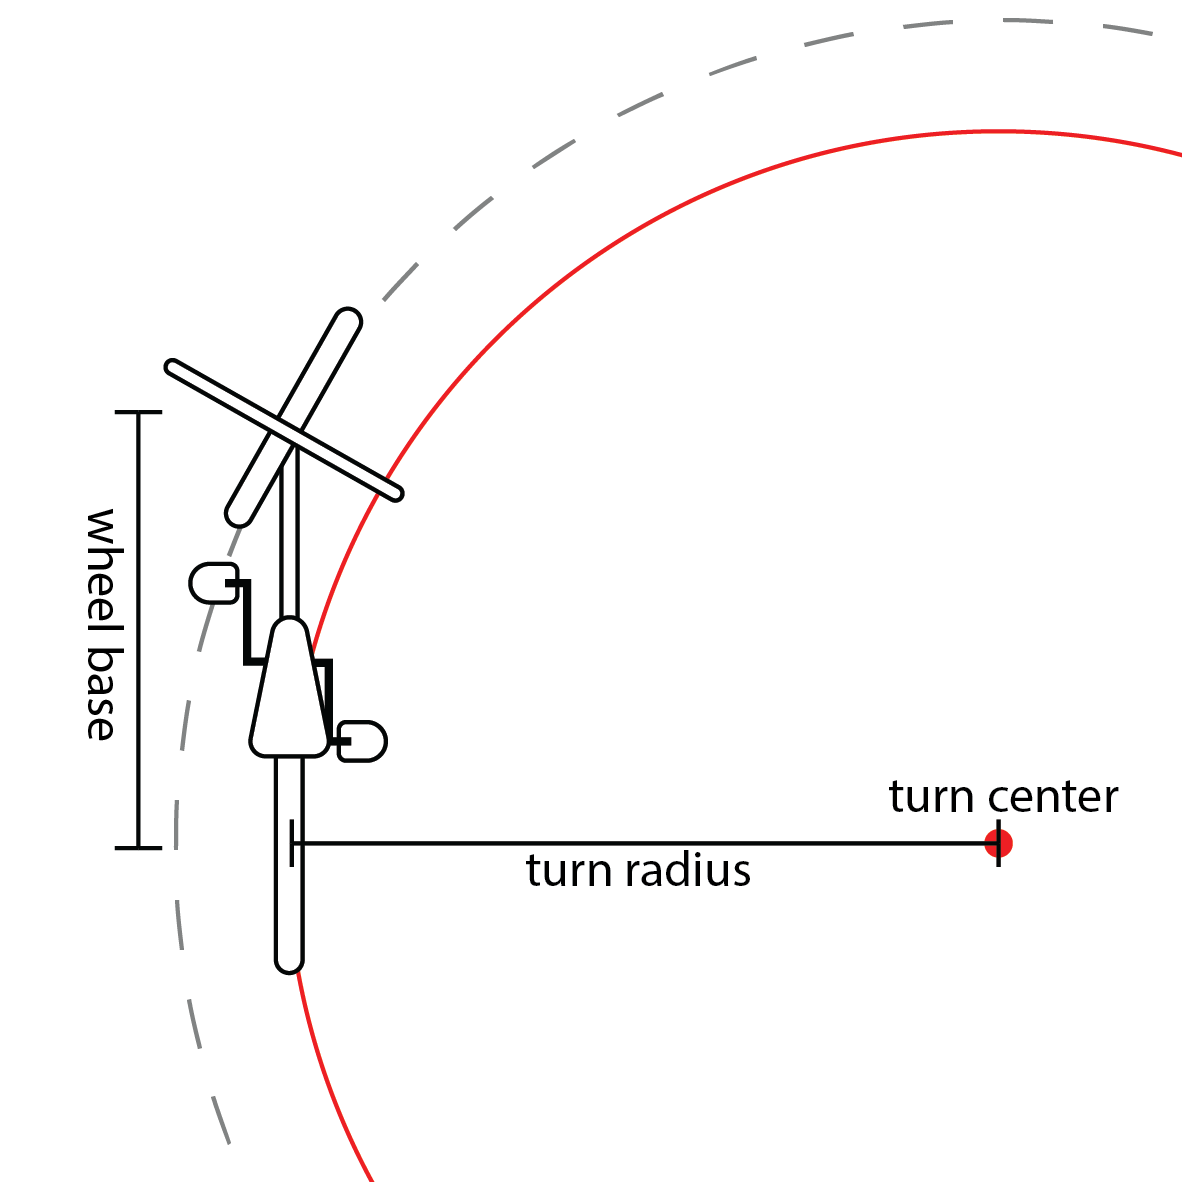
\includegraphics[width=0.5\textwidth]{images/turningDiagram.png}
	\caption{basic turn geometry}
\end{figure}

The wheelbase variable in the code is the distance between the center of both the front and rear axle of the bike, while sign is the direction of the turn (left or right).
\begin{CsCode}
else//Curve
	{
		float turnRadius = wheelbase / (Mathf.Sin(Mathf.Abs(steeringAngle) * Mathf.Deg2Rad));
		int sign = steeringAngle < 0 ? -1 : 1;
		Vector3 turningCurveCenter = (transform.position + (transform.right.normalized * sign * turnRadius));
		bike.transform.RotateAround(turningCurveCenter, Vector3.up, sign * ((speedInMetersPerSecond * 1f) / (2f * Mathf.PI * turnRadius) * 360f) * Time.deltaTime);

		tilt = Mathf.Atan((speedInMetersPerSecond * speedInMetersPerSecond) / (turnRadius * Physics.gravity.y)) * Mathf.Rad2Deg * sign * tiltFactor;
	}
\end{CsCode}
The tilting of the bike is also calculated in order to have a more realistic turn and is based on the following formula:

\begin{equation}
\text{tilt} = \text{Atan}(\frac{\text{speed}^2}{\text{turnRadius} * \text{g}}) * \text{sign} * \text{tiltFactor}
\end{equation}

The value of the tilt factor can be set in the Unity editor depending on how exaggerated the tilting should be.
If the bike is going straight then the tilt is 0.
To further improve the tilting, the tilting was also smoothed via lerping.
\begin{CsCode}
	float lastSmoothTilt = smoothTilt;
	smoothTilt = Mathf.Lerp(smoothTilt, tilt, Time.deltaTime * 30f);
	bike.transform.localEulerAngles = new Vector3(bike.transform.localEulerAngles.x, bike.transform.localEulerAngles.y, smoothTilt);
\end{CsCode}
After the bike position and rotation have been updated the position and rotation of the "XR Origin" also need to be changed accordingly.
To update the position of the "XR Origin" the "VR Player Position" game object which is attached the "City Bike" is used.  Since the "VR Player Position" is a child of the main bike game object they share their position.
 The position and rotation are again smoothed by lerping in an effort to reduce motion sickness and camera jittering.
\begin{CsCode}
	//Moving and turning the VR Player with the bike
	//Smoothing VR Camera transforms slightly to reduce jitter and motion sickness
	VRCamera.transform.position = Vector3.Lerp(VRCamera.transform.position, vRPlayerPositionTransform.position, Time.deltaTime * 30f);
	smoothBikeRotation = Quaternion.Lerp(smoothBikeRotation, bike.transform.rotation, Time.deltaTime * 20f);
	float deltaBikeRotationY = smoothBikeRotation.eulerAngles.y - lastBikeRotationY;
	lastBikeRotationY = smoothBikeRotation.eulerAngles.y;
	Vector3 vrRotation = VRCamera.transform.rotation.eulerAngles;
	float smoothTiltDelta = smoothTilt - lastSmoothTilt;
	VRCamera.transform.rotation = Quaternion.Euler(vrRotation.x, vrRotation.y + deltaBikeRotationY, vrRotation.z);
\end{CsCode} 

%%%-----------------------------------------------------------------------------
\chapter{Summary}
%%%-----------------------------------------------------------------------------

Based on the aims defined in chapter \ref{chapAims} the following goals were accomplished:
\begin{itemize}
	\item A hard and software architecture for the bicycle simulator were defined
	\item The bike was successfully mounted onto the smart trainer
	\item Sensor data from the hall effect sensor are successfully gather and used for braking. 
	\item Steering via an Oculus controller was implemented as well as a possibility to use a gyroscope sensor in the future.
	\item A small test ground in the form of a parking lot was created.
	\item Tilting and camera smoothing were implemented in order to combat motion sickness.
\end{itemize}
Therefore, six of the seven goals were successfully achieved. 
Unfortunately due to time constrains no user study was conducted. 
However, the bicycle simulator will be displayed at the MTD + DA + IM project showcase, were students can try out it.
All in all a lot has been achieved considering the delayed start of the project as well as the problems faced with the Arduino and the bike cassette.
Taking all of this into account here are various aspects of the bike simulator that can be improved in a future project:
\begin{itemize}
	\item Higher quality and more diverse environments for driving bike around.
	\item Fully implementing the gyroscope sensor.
	\item Proper mounting and fixing position of sensor and Oculus controller
	\item Moving calculations from the Arduino code into the Unity code to save on memory space.
	\item Fine-tuning various variables in Unity like the tilt factor to decrease motion sickness in users.
\end{itemize}

%%%-----------------------------------------------------------------------------
\appendix                                                   % Switch to appendix
%%%-----------------------------------------------------------------------------

%%%-----------------------------------------------------------------------------
\chapter{Supplementary Materials}
%%%-----------------------------------------------------------------------------



%%%-----------------------------------------------------------------------------
\MakeBibliography[nosplit]
%%%-----------------------------------------------------------------------------

%%%-----------------------------------------------------------------------------
\end{document}
%%%-----------------------------------------------------------------------------
